%!TEX root = ../main.tex
We have already introduced two kind of dual spaces, we will develop those notions and the properties which they imply. 

Moreover we will introduce the notion of reflexivity which is a crucial property to develop more tools for applications.

\subsubsection{Dual spaces}
Recalling the definition \vref{defn-dual-star}, given the normed vector space $X$, its \emph{topological dual space} is the space of all linear bounded functional $T: X \to \RR$, namely:
$$
	X^\star
	\coloneqq \Bc(X,\RR) 
	= \{T\in\Lc(X, \RR): \quad T \text{ bounded}\}
,
$$
and its norm is:
$$
	\norm{L}_\star 
	\coloneqq \sup_{\norm{x}_X=1} |Lx|
.
$$
Notice that $X^\star$ is always a Banach space (see theorem \vref{theo-Bc-banach}).

Now consider the following two results which we will use them later.

\begin{prop}\label{x-y-isomorphic-dual}
	If $X$ and $Y$ are isomorphic normed vector spaces, then $X^\star$ and $Y^\star$ are isomorphic.
\end{prop}
\begin{proof}
	Consider an isomorphism $J: X \to Y$.
	
	Give $L \in X^\star$ and define:
	$$\Lambda y = L J^{-1} y \quad \forall y \in Y.$$
	
	Thus we have a linear map $\tilde J: X^\star \to Y^\star$ by setting:
	$$\tilde J L = \Lambda \quad \forall L \in X^\star.$$
	
	Now it's easy to prove that $\tilde J$ is bounded, injective and surjective.
	
	Therefore, thanks to the bounded inverse mapping theorem (see \vref{bounded-inverse-theo}), we have that $\tilde J$ is an isomorphism.	
\end{proof}

Moreover, the following proposition holds.
\begin{prop}
	If $X$ is infinite dimensional, then $X^\star \subsetneq X'$.
\end{prop}

\paragraph{Characterization of linear bounded functionals}
\begin{theo}
	Let $L \in X'$ such that $L \neq 0$.\\
	Then the following statements are equivalent:
	\begin{enumerate}
		\item $L \in  X^\star$;
		\item $\Ker(L)$ is closed;
		\item $\overline{\Ker(L)} \subsetneq X$, that is $\Ker{L}$ is not dense in $X$.
	\end{enumerate}
	\label{theo-charact-bdd-functionals}
\end{theo}
\begin{proof} We prove the pairwise implications.
	
	\textit{Proof of $L \in X^\star$ implies $\Ker(L)$ is closed}:\\
	Take a sequence $x_{n}$ belonging to the Kernel, that is, $Lx_{n}=0$, converging to some $x$. We want to show that $Lx=0$, but since $L$ is bounded (i.e. continuous), this is a sequence of zeros which converges to $0$, hence $L(0)=0$, so $x\in \Ker(L)$.
	
	\textit{Proof of $\Ker(L)$ is closed implies $\Ker{L}$ is not dense in $X$}:\\	
	By contradiction, suppose $\overline{\Ker(L)} =X$. As $\Ker(L)$ is closed by hypothesis we have $\Ker(L) = X$, but then it would be $L \equiv 0$, which goes against the hypothesis.
	
	\textit{Proof of $\Ker{L}$ is not dense in $X$ implies $L \in X^\star$}:\\	
	Again by contradiction, let $L \notin X^\star$, and $x \in X$ such that $Lx = \alpha \neq 0$, namely $x \notin \Ker(L)$.\\	
	Let $\eps > 0$. Since $L \notin X^\star$, namely $L$ is unbounded, then $\exists \, y \in B(0,\eps)$ such that $Ly = \beta$ with $|\beta|>|\alpha|$.\\
	Set $\gamma = -\frac \alpha \beta$: we have $|\gamma|<1$.\\
	Observe now that 
	$$
		L(x + \gamma y) 
		= Lx + \gamma Ly 
		= 0
		,
	$$ and thus $z = x+\gamma y \in \Ker(L)$, with $z \in B(x,\eps)$.\\
	\begin{figure}[htpb]
		\centering
		\tikzset{every picture/.style={line width=0.75pt}} %set default line width to 0.75pt        
		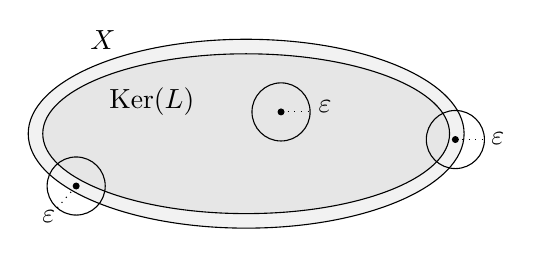
\begin{tikzpicture}[x=0.75pt,y=0.75pt,yscale=-0.7,xscale=0.7]
		%uncomment if require: \path (0,300); %set diagram left start at 0, and has height of 300

		\draw   (374,129) .. controls (374,117.95) and (382.95,109) .. (394,109) .. controls (405.05,109) and (414,117.95) .. (414,129) .. controls (414,140.05) and (405.05,149) .. (394,149) .. controls (382.95,149) and (374,140.05) .. (374,129) -- cycle ;
		\draw  [dotted]  (394,129) -- (414,129) ;
		\draw  [fill={rgb, 255:red, 0; green, 0; blue, 0 }  ,fill opacity=0.05 ] (100,125) .. controls (100,89.1) and (167.16,60) .. (250,60) .. controls (332.84,60) and (400,89.1) .. (400,125) .. controls (400,160.9) and (332.84,190) .. (250,190) .. controls (167.16,190) and (100,160.9) .. (100,125) -- cycle ;
		\draw  [fill={rgb, 255:red, 0; green, 0; blue, 0 }  ,fill opacity=0.05 ] (110,125) .. controls (110,94.62) and (172.68,70) .. (250,70) .. controls (327.32,70) and (390,94.62) .. (390,125) .. controls (390,155.38) and (327.32,180) .. (250,180) .. controls (172.68,180) and (110,155.38) .. (110,125) -- cycle ;
		\draw  [fill={rgb, 255:red, 0; green, 0; blue, 0 }  ,fill opacity=1 ] (392,129) .. controls (392,127.9) and (392.9,127) .. (394,127) .. controls (395.1,127) and (396,127.9) .. (396,129) .. controls (396,130.1) and (395.1,131) .. (394,131) .. controls (392.9,131) and (392,130.1) .. (392,129) -- cycle ;
		\draw   (113,161) .. controls (113,149.95) and (121.95,141) .. (133,141) .. controls (144.05,141) and (153,149.95) .. (153,161) .. controls (153,172.05) and (144.05,181) .. (133,181) .. controls (121.95,181) and (113,172.05) .. (113,161) -- cycle ;
		\draw  [dotted]  (120,176) -- (133,161) ;
		\draw  [fill={rgb, 255:red, 0; green, 0; blue, 0 }  ,fill opacity=1 ] (131,161) .. controls (131,159.9) and (131.9,159) .. (133,159) .. controls (134.1,159) and (135,159.9) .. (135,161) .. controls (135,162.1) and (134.1,163) .. (133,163) .. controls (131.9,163) and (131,162.1) .. (131,161) -- cycle ;
		\draw   (254,110) .. controls (254,98.95) and (262.95,90) .. (274,90) .. controls (285.05,90) and (294,98.95) .. (294,110) .. controls (294,121.05) and (285.05,130) .. (274,130) .. controls (262.95,130) and (254,121.05) .. (254,110) -- cycle ;
		\draw  [dotted]  (274,110) -- (294,110) ;
		\draw  [fill={rgb, 255:red, 0; green, 0; blue, 0 }  ,fill opacity=1 ] (272,110) .. controls (272,108.9) and (272.9,108) .. (274,108) .. controls (275.1,108) and (276,108.9) .. (276,110) .. controls (276,111.1) and (275.1,112) .. (274,112) .. controls (272.9,112) and (272,111.1) .. (272,110) -- cycle ;

		\draw (417,122.4) node [anchor=north west][inner sep=0.75pt]    {$\varepsilon $};
		\draw (141,52.4) node [anchor=north west][inner sep=0.75pt]    {$X$};
		\draw (154,91.4) node [anchor=north west][inner sep=0.75pt]    {$\mathrm{Ker}( L)$};
		\draw (108,176.4) node [anchor=north west][inner sep=0.75pt]    {$\varepsilon $};
		\draw (298,100.4) node [anchor=north west][inner sep=0.75pt]    {$\varepsilon $};
		\end{tikzpicture}
	\end{figure}
	\FloatBarrier
	Then\footnote{Remember that saying that $\forall x\in X,\forall \varepsilon  >0,\exists \, z\in \Ker(L) ,z\in B( x,\varepsilon )$ is a way to say that $\Ker(L)$ is dense in $X$.} $\overline{\Ker(L)}=X$, which is a contradiction.
\end{proof}


\paragraph{Duality in $L^p$ spaces} The following two theorems, the first for the case $p \in (1, \infty)$ and the second for the case $p=1$, discuss duality for functional spaces $L^p$.

Notice that if we are working on $L^p$, with $p \in (1, \infty)$, then we can find $g \in L^q$ for which
$$
	Lg(f)
	= \int_\Omega f g \, \dmu
	\quad \text{where }Lg \in (L^p)^\star
	.
$$

The following theorem goes further providing a complete characterization.

\begin{theo}\label{theo-duality-l-p-1-infinity}
	Let $(\Omega, \mm, \mu)$ a complete measure space.\\
	Consider $L^p(\Omega, \mm,\mu)$ for any fixed $p \in (1, \infty)$.\\
	If $\Lambda \in (L^p(\Omega, \mm, \mu))^\star$ then there exists a unique $g \in L^q(\Omega, \mm, mu)$ where $q$ is the conjugate index of $p$, such that:
	$$\Lambda (f) = \int_\Omega f g \dmu \quad \forall f \in L^p(\Omega, \mm, \mu).$$
	Moreover, we have:
	$$\norm{\Lambda}_{(L^p(\Omega, \mm, \mu))^\star} = \norm{g}_{L^q(\Omega, \mm, \mu)}.$$
	Hence $(L^p(\Omega, \mm, \mu))^\star$ and $L^q(\Omega, \mm, \mu)$ are isometrically isomorphic through $T: \Lambda \mapsto g$.
\end{theo}

This one instead develops the case in which $p = 1$ and $q = \infty$.

\begin{theo}\label{theo-duality-l-p-1}
	Let $\Omega \in \Lc(\RR^N)$ and consider $L^1(\Omega, \Lc(\Omega), \lambda)$.\\
	If $\Lambda \in (L^1(\Omega, \mm, \mu))^\star$ then there exists a unique $g \in L^\infty(\Omega, \mm, \mu)$ such that:
	$$\Lambda (f) = \int_\Omega f g \dmu \quad \forall f \in L^1(\Omega, \Lc(\Omega), \lambda).$$
	Moreover, we have:
	$$\norm{\Lambda}_{(L^1(\Omega, \Lc(\Omega), \lambda))^\star} = \norm{g}_{L^\infty(\Omega, \Lc(\Omega), \lambda)}.$$
	Hence $(L^1(\Omega, \mm, \mu))^\star$ and $L^\infty(\Omega, \mm, \mu)$ are isometrically isomorphic through $T: \Lambda \mapsto g$.
\end{theo}

Pay attention to the main difference: the second result only holds in $\RR^N$ with the Lebesgue measure, while the first one holds in a general metric space.

We need more tools to discuss the case $p=\infty$, we will come back to this at page \pageref{paragraph-duality-p-infinity}.
